\documentclass[12pt,a4paper,onecolumn]{exam}
\usepackage{amsmath}
\usepackage{amssymb}
\usepackage{graphicx}
\usepackage{float}
\usepackage{geometry}
\usepackage{tikz}
\usepackage[skins]{tcolorbox} % Use [skins] to get the rounded shape

% --- Define our simple \questionheader command ---
\newcommand{\questionheader}[1]{%
  \begin{tcolorbox}[
    enhanced,
    colback=black,
    coltext=white,
    boxrule=0pt,              
    fontupper=\Large\bfseries, 
    arc=4mm                   
  ]
  #1 
  \end{tcolorbox}%
}
% --- End of definition ---
\newtcolorbox{answerbox}[1]{
  boxrule=0.4pt,   % Sets the thickness of the border
  colback=white,   % Sets the background color
  height=#1,       % <-- Use the first argument (#1) as the height
}


\usepackage[font = small]{caption}
\usepackage{subcaption}

\newenvironment{blanksolution}
  {%
    \renewcommand{\solutiontitle}{\noindent}%
    \begin{solution}%
  }%
  {\end{solution}}  
\usepackage{listings}

\lstset{
    language=Python,
    basicstyle=\ttfamily, 
    }

\begin{document}

\begingroup  
    \centering
    \LARGE E9 241 Digital Image Processing\\
    \LARGE Assignment 3\\[0.5em]
    \large \today\\[0.5em]
    \large Dwaipayan Haldar\par
\endgroup
\noindent\rule{\textwidth}{0.5pt}
\printanswers
\renewcommand{\solutiontitle}{\noindent\textbf{Ans:}\enspace}

\questionheader{1. Directional Filtering}

\begin{solution}
\begin{itemize}
    \item[(a)] 
The image consists of three sin waves. The DFT results are as expected. Since DFT is conjugate symmetric so, there are 6 impulses(3 for the 3 sin wave, and 3 for its conjugate symmetric component). $x_1(m,n)$ has a frequency index of 12. There are indeed two white dot or impulse at $\pm 12$ from the center along the vertical axis. $x_2(m,n)$ has a frequency index of 8 along the horizontal. So there are two dots along the horizontal from the center at $\pm 8$. The third component $x_3(m,n)$ has a frequency index of 6 along the vertical and 10 along horizontal. So, there are two dots at $\pm(10,6)$. 
\end{itemize}
        \begin{figure}[H]
        \centering
        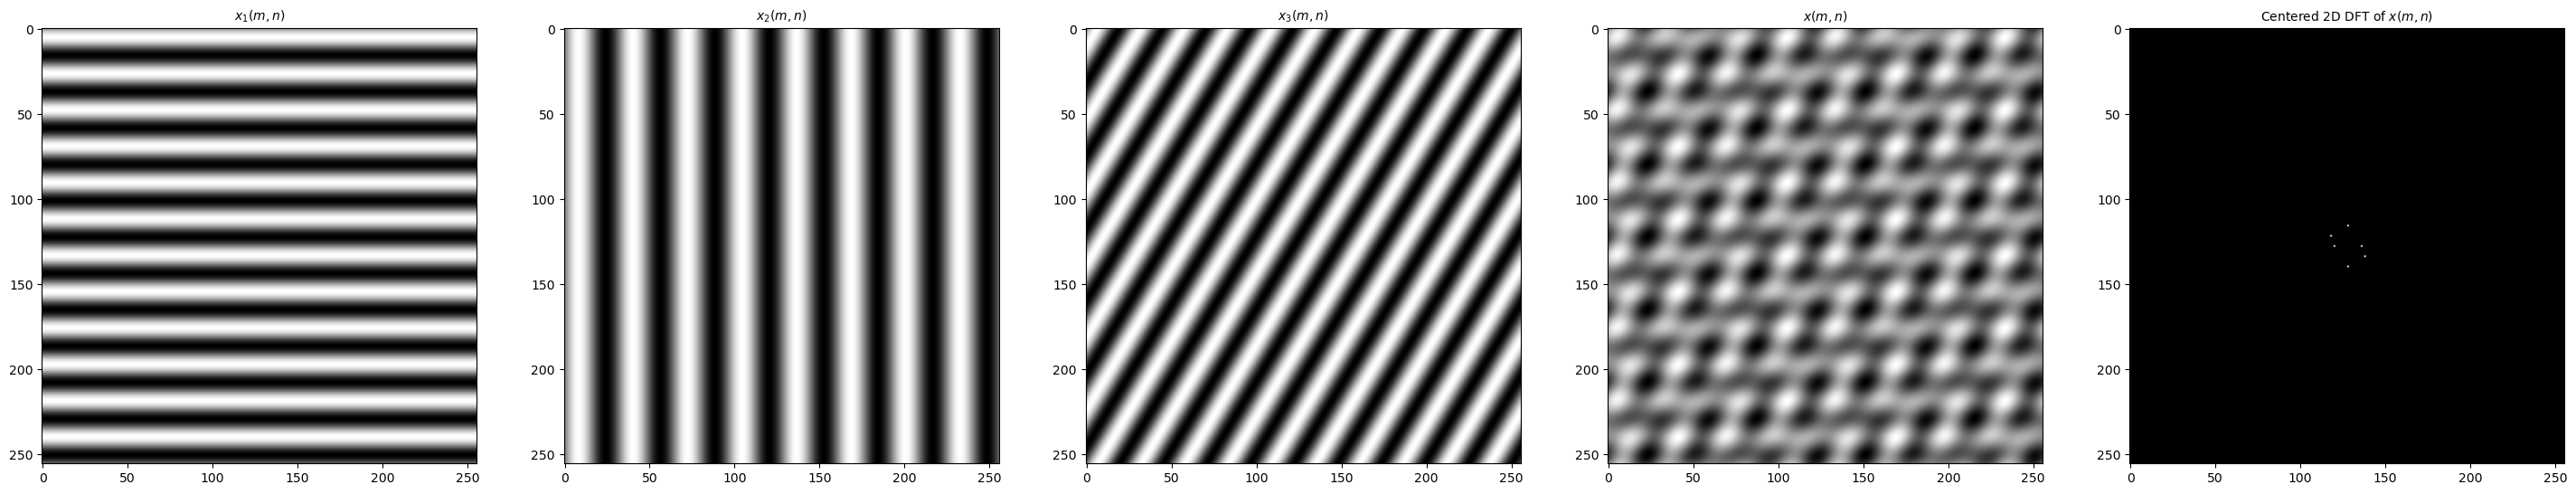
\includegraphics[scale = .18]{Output_Images/P01a.png}
        \caption{Problem 1.(a) image consists of 3 sin waves, combined average image and the centered DFT of the combined image}
        \label{fig:1a}
        \end{figure}

\begin{itemize}
    \item[(b)] Analyzing the results for the first filter:\\
    $H_1(u,v)= H(u,v; -20 ^{\circ},20^{\circ})$. \\
    This filter retains one side of the sin wave $x_2(m,n) = sin(\frac{2\pi \cdot 8n}{M})$. All the other sin waves are completely removed, as a result that did not show up in the result. Now for $x_2(m,n)$ this operation of retaining only one impulse out of the two can be seen as retaining only one complex exponential in the time domain. We can analyze this as follows:
\[
\begin{aligned}
x_2(m,n) &= \sin\left(\frac{2\pi \cdot 8n}{M}\right)
          = \frac{1}{2j}\left(e^{j\frac{2\pi \cdot 8n}{M}} - e^{-j\frac{2\pi \cdot 8n}{M}}\right) \notag \\
          & \updownarrow \notag\\
X_2(u,v) &= \frac{M}{2j}\big(\delta(v-8) - \delta(v+8)\big) \notag
\end{aligned}
\]
Now if we remove the negative impulse in the frequency domain, we are basically removing a complex exponential in the time domain. The equivalent $\hat x_2(m,n)$ we can express as:

\[
\begin{aligned}
\hat X_2(u,v) &= \frac{M}{2j}\delta(v-8) \notag \\
 & \updownarrow \notag\\
\hat x_2(m,n) &= \sin\left(\frac{2\pi \cdot 8n}{M}\right)
          = \frac{1}{2j}e^{j\frac{2\pi \cdot 8n}{M}} \notag
\end{aligned}
\]
now if we take the real part of $\hat x_2(m,n)$, we will get $$Re\left(\frac{1}{2j}e^{j\frac{2\pi \cdot 8n}{M}}\right) =  \frac{1}{2}sin\left(\frac{2\pi \cdot 8n}{M}\right) = \frac{1}{2}x_2(m,n)$$ 
Since, the combined image was originally $\frac{x_1(m,n)+x_2(m,n)+x_3(m,n)}{3}$. So the output should come out as $\frac{1}{6}sin\left(\frac{2\pi \cdot 8n}{M}\right)$ which is indeed the result in Fig. \ref{fig:1bi}

        \begin{figure}[H]
        \centering
        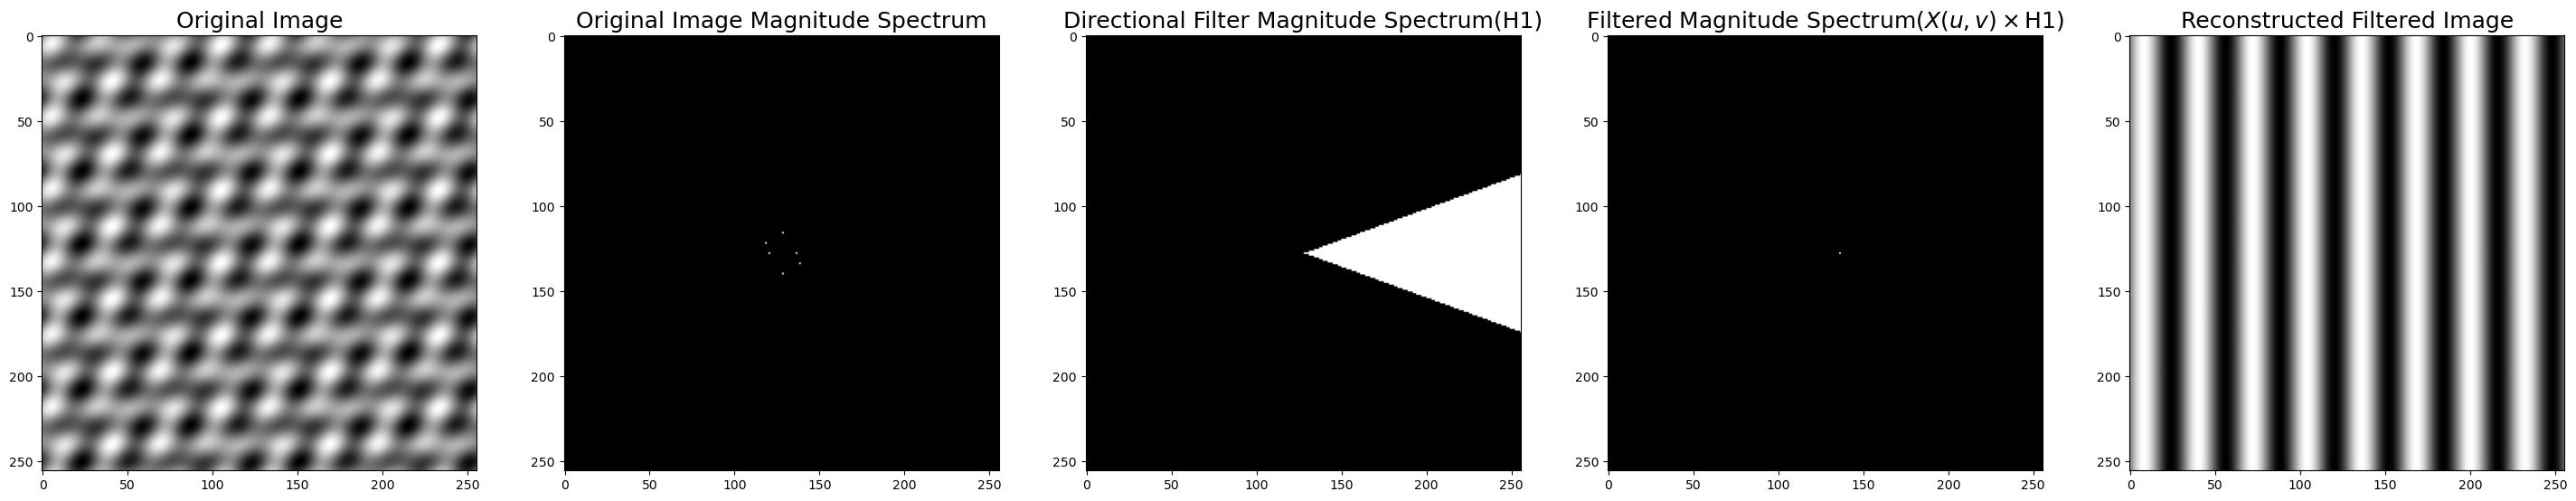
\includegraphics[scale = .18]{Output_Images/P01bi.png}
        \caption{(From Left) (i) $x(m,n)$; (ii) $|X(u,v)|$; (iii) $|H_1(u,v)|$; (iv) $|X(u,v) \times H_1(u,v)|$; (v) $\frac{x_2(m,n)}{6}$}
        \label{fig:1bi}
        \end{figure}

For all the other cases, same analysis will suffice. For $H_2$, the output will be $\frac{x_1(m,n)}{6}$ (Fig. \ref{fig:1bii}). For $H_3$, the output will be $\frac{x_3(m,n)} {6}$ (Fig. \ref{fig:1biii}) and for $H_4$, the output will be $\frac{x(m,n)}{2}$ (Fig. \ref{fig:1biv}).

        \begin{figure}[H]
        \centering
        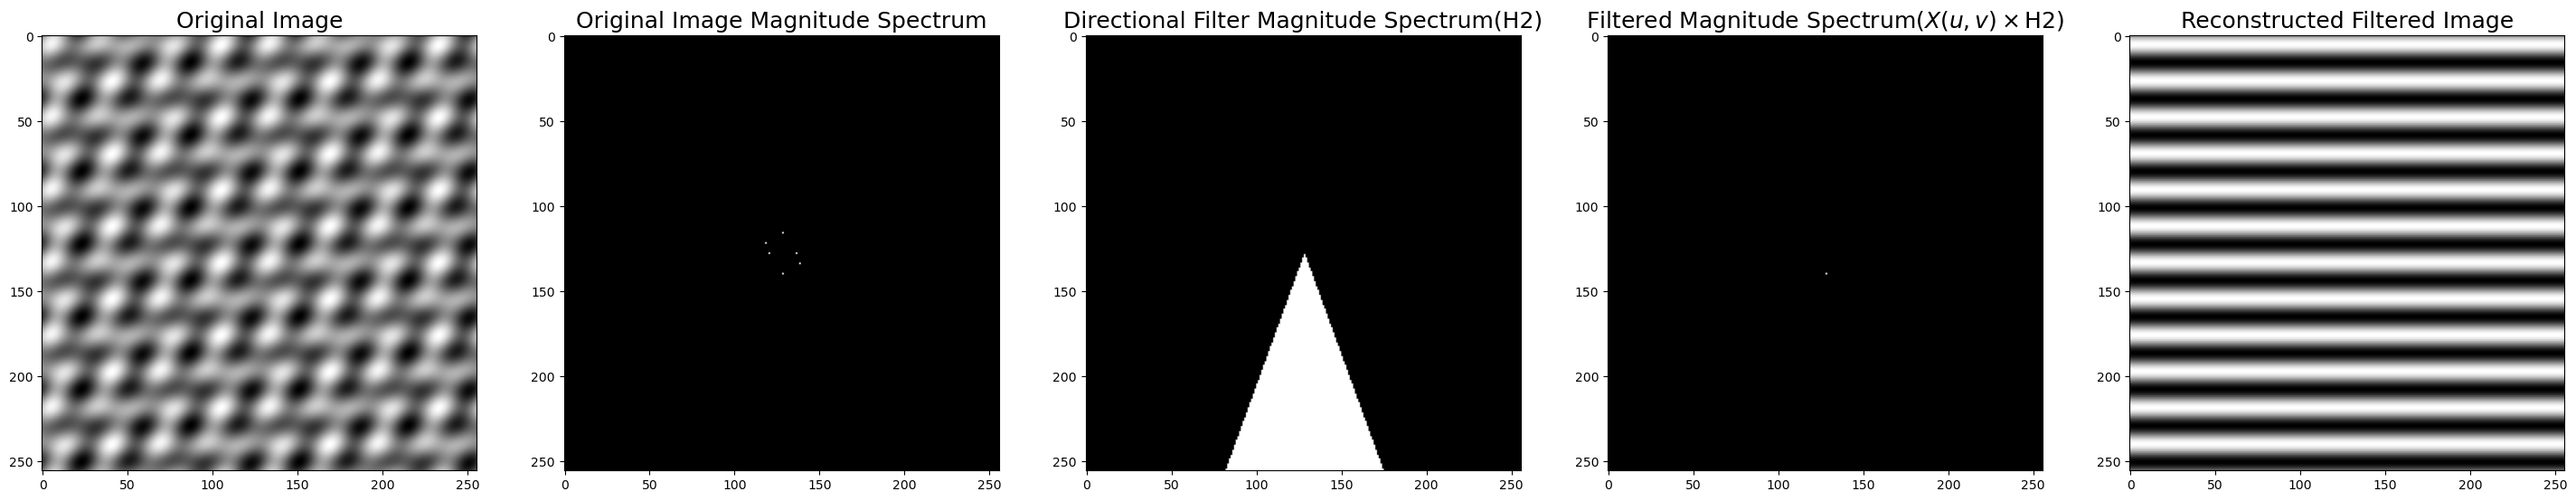
\includegraphics[scale = .18]{Output_Images/P01bii.png}
        \caption{(From Left) (i) $x(m,n)$; (ii) $|X(u,v)|$; (iii) $|H_2(u,v)|$; (iv) $|X(u,v) \times H_2(u,v)|$; (v) $\frac{x_1(m,n)}{6}$}
        \label{fig:1bii}
        \end{figure}

        \begin{figure}[H]
        \centering
        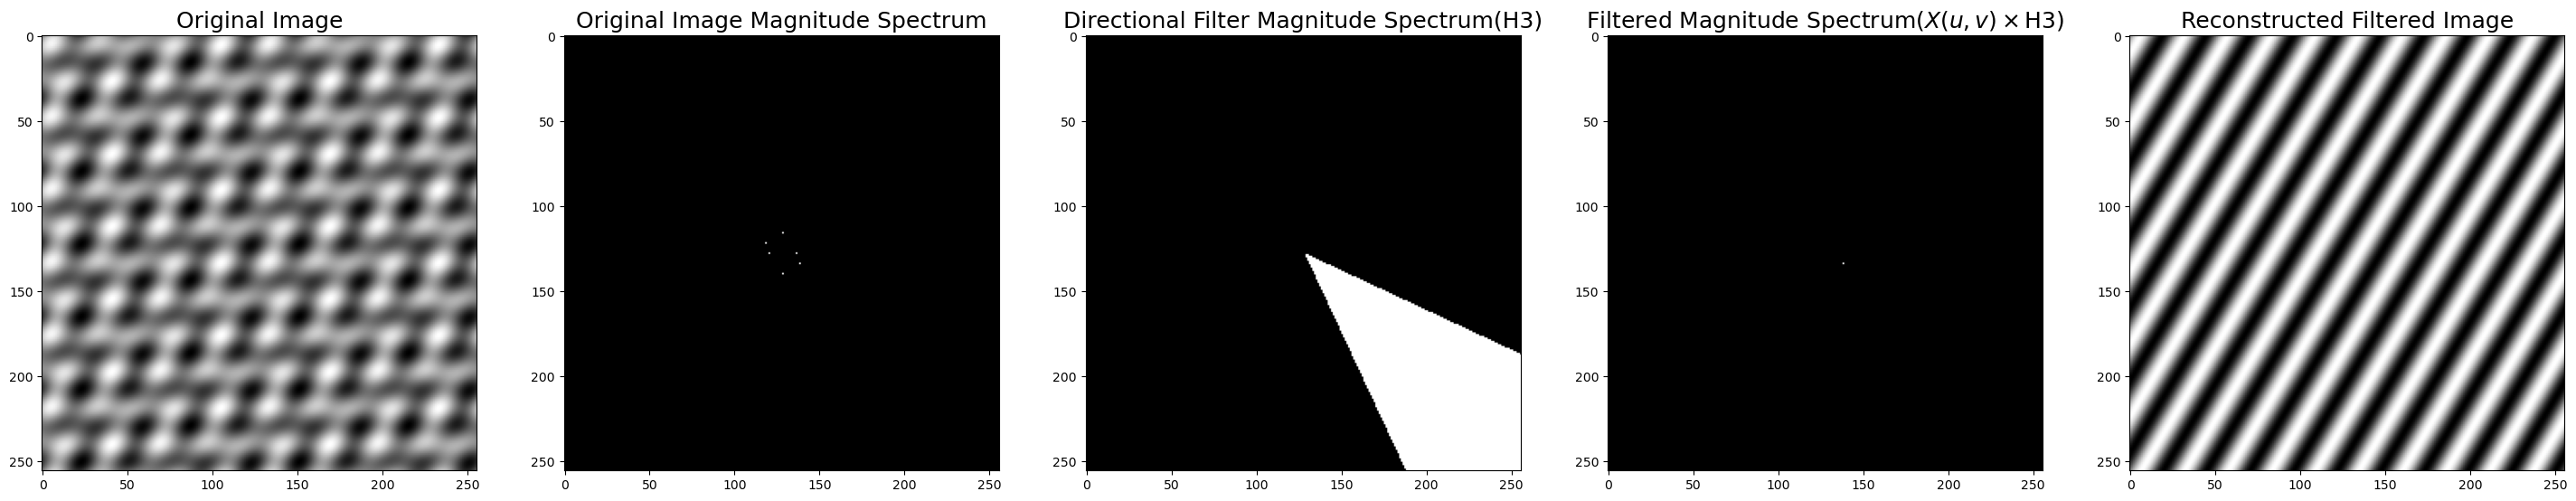
\includegraphics[scale = .18]{Output_Images/P01biii.png}
        \caption{(From Left) (i) $x(m,n)$; (ii) $|X(u,v)|$; (iii) $|H_3(u,v)|$; (iv) $|X(u,v) \times H_3(u,v)|$; (v) $\frac{x_3(m,n)}{6}$}
        \label{fig:1biii}
        \end{figure}

        \begin{figure}[H]
        \centering
        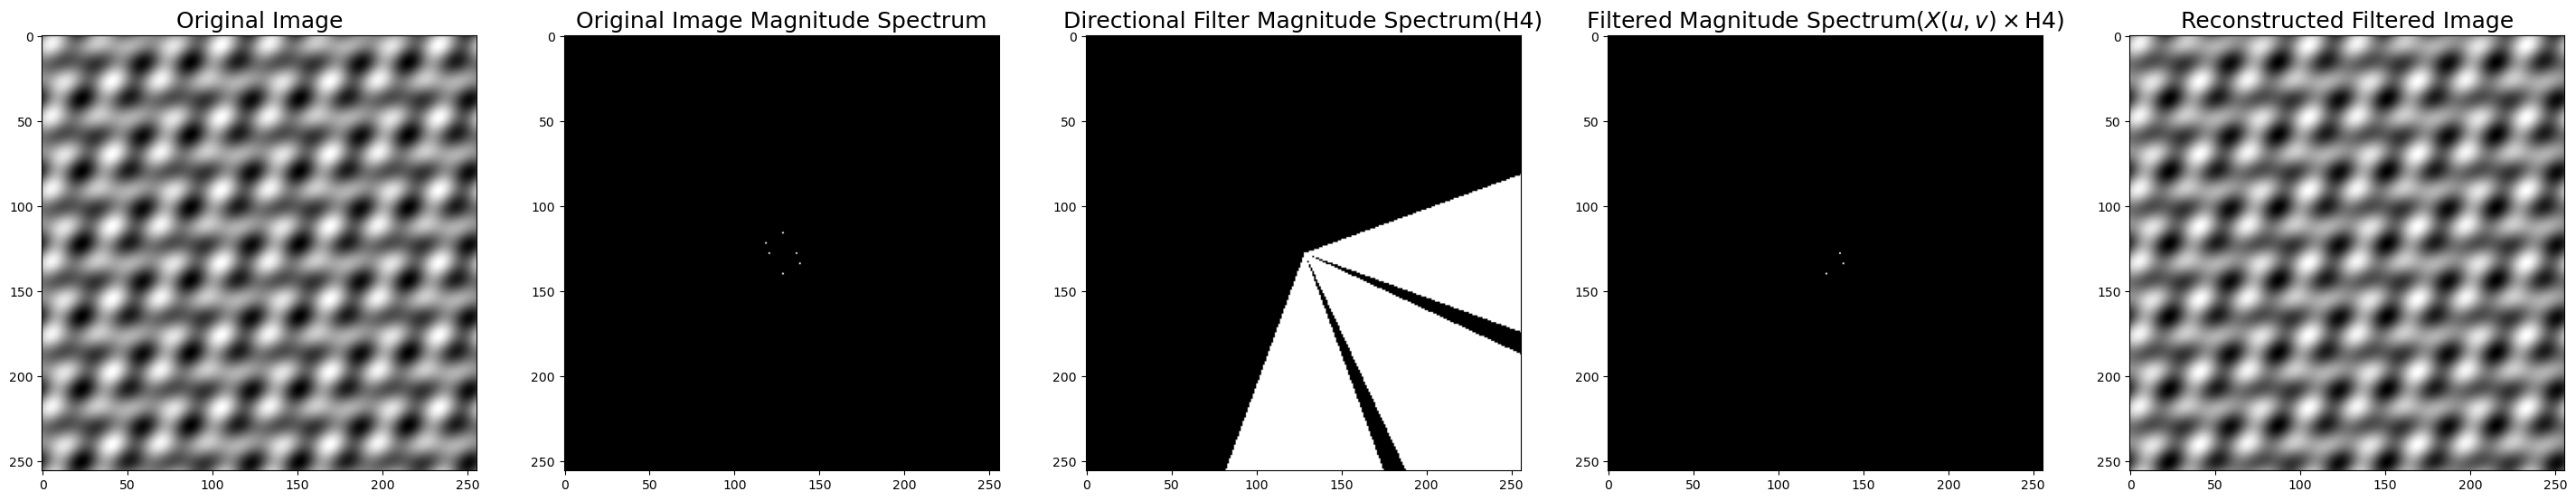
\includegraphics[scale = .18]{Output_Images/P01biv.png}
        \caption{(From Left) (i) $x(m,n)$; (ii) $|X(u,v)|$; (iii) $|H_4(u,v)|$; (iv) $|X(u,v) \times H_4(u,v)|$; (v) $\frac{x(m,n)}{2}$}
        \label{fig:1biv}
        \end{figure}


\item[(c)] The MSE values for the different filters are as follows:
\[
\begin{aligned}
  MSE(H_1) = 0.125 \\
  MSE(H_2) = 0.125 \\
  MSE(H_3) = 0.125 \\
  MSE(H_4) = 0.0416 \\
\end{aligned}
\]

As per our calculation shown in part (b), the $$MSE(H_1) = \frac{1}{M^2}\sum_{m=0}^{255}\sum_{n=0}^{255}(x(m,n)-\frac{1}{6}x_2(m,n))^2 $$ which is indeed 0.125. It is calculated in the next code block in the \verb|wrapper.ipynb| file. Similarly, for the other filters, the theoretical values of the MSE can be shown as:
\[
\begin{aligned}
  MSE(H_3) = \frac{1}{M^2}\sum_{m=0}^{255}\sum_{n=0}^{255}(x(m,n)-\frac{1}{6}x_3(m,n))^2 = 0.125 \\
  MSE(H_2) = \frac{1}{M^2}\sum_{m=0}^{255}\sum_{n=0}^{255}(x(m,n)-\frac{1}{6}x_1(m,n))^2 = 0.125 \\
  MSE(H_4) = \frac{1}{M^2}\sum_{m=0}^{255}\sum_{n=0}^{255}(x(m,n)-\frac{1}{2}x(m,n))^2 = 0.0416 \\
\end{aligned}
\]
$H_4$ has the least MSE as expected because it is the same output with a scale factor of 0.5. Visually, it is exactly the same. 


\end{itemize}
\end{solution}


\questionheader{2. Gaussian Blurring and Inverse Filtering}

\begin{solution}
  
  \begin{itemize}
    \item[(a)] A gaussian kernel of size $13 \times 13$ is created. The kernel must be padded with zeros otherwise it cannot be operated with in the frequency domain. To avoid the circular convolution artifacts it is padded to $(image size + kernel size -1) = 1024+13-1 = 1036$. So the kernel is padded to $1036 \times 1036$ size. Similarly, the image is also padded. For the kernel the $(0,0)$ is at the center but the \verb|fft| algorithm expects that to be in the top left corner. So a \verb|ifftshift| is done before \verb|fft|. Then the filter frequency domain response is multiplied with image frequency domain response and inverse is done to get the output as in Fig.\ref{fig:2a}. 
    
        \begin{figure}[H]
        \centering
        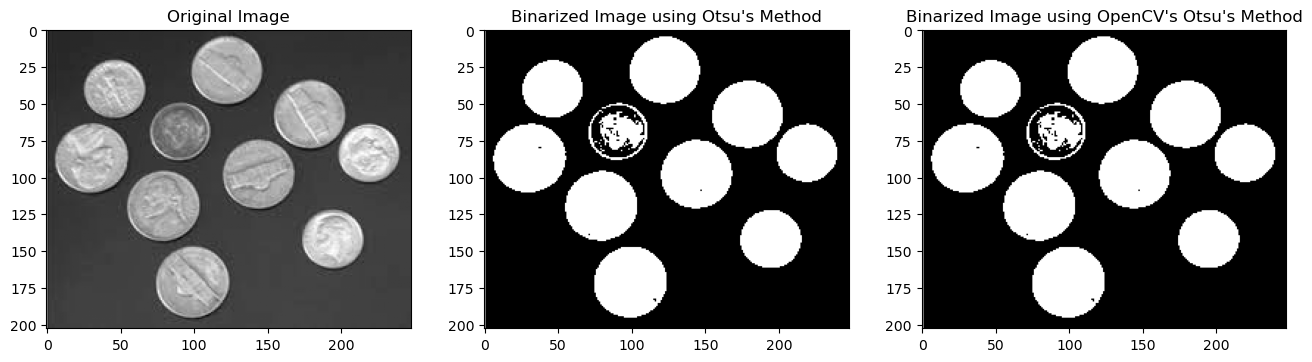
\includegraphics[scale = .18]{Output_Images/P02a.png}
        \caption{Original Image and the filtered image (Filtered with spatial domain gaussian filter in frequency domain)}
        \label{fig:2a}
        \end{figure}

    \item[(b)] 
    \begin{itemize}
      \item[(i)] The DFT of Gaussian kernel is also a Gaussian but with inverse spread. That is why the Centered DFT of Gaussian kernel($13 \times 13$) in Fig.\ref{fig:2b} has much less spread than the spatial domain kernel which is 2.5 as given in the problem. Actually here the spread is 0.75.
      \item[(ii)] The inverse of the DFT in (i) is quite obvious. No special observation in this case.
      \item[(iii)] The DFT of the padded kernel is plotted. Here ripples are visible. The reason can be explained as follows: \\
         $1036 \times 1036$ zero padded kernel can be seen as a $1036 \times 1036$ Gaussian kernel multiplied with a box function with a dimension of $13 \times 13$. This is in the frequency domain is convolution of Gaussian with Sinc function. That Sinc function results in those ripples that are visible.  
        \item[(iv)] It is just the inverse of the function in (iii). Here the ripples are yet more visible since the whole filter is inverted. 
      \end{itemize}

      \item[(c)] The frequency domain gaussian is defined and then optimal k  and minimum error for the optimal k is found out, which are: $$k_{\text{optimal}} = 0.00013, \quad \text{Error}_{\text{min}} = 7.689$$ The Gaussian fit and the inverse gaussian fit is plotted in Fig.\ref{fig:2c}. One important observation in this context is that there are no ripples in the Gaussian fit. Since it is purely Gaussian and does not intermix the property of Gaussain and Sinc function which occured in the case of the $13 \times 13$ kernel due to the presence of box function. 
        \begin{figure}[H]
        \centering
        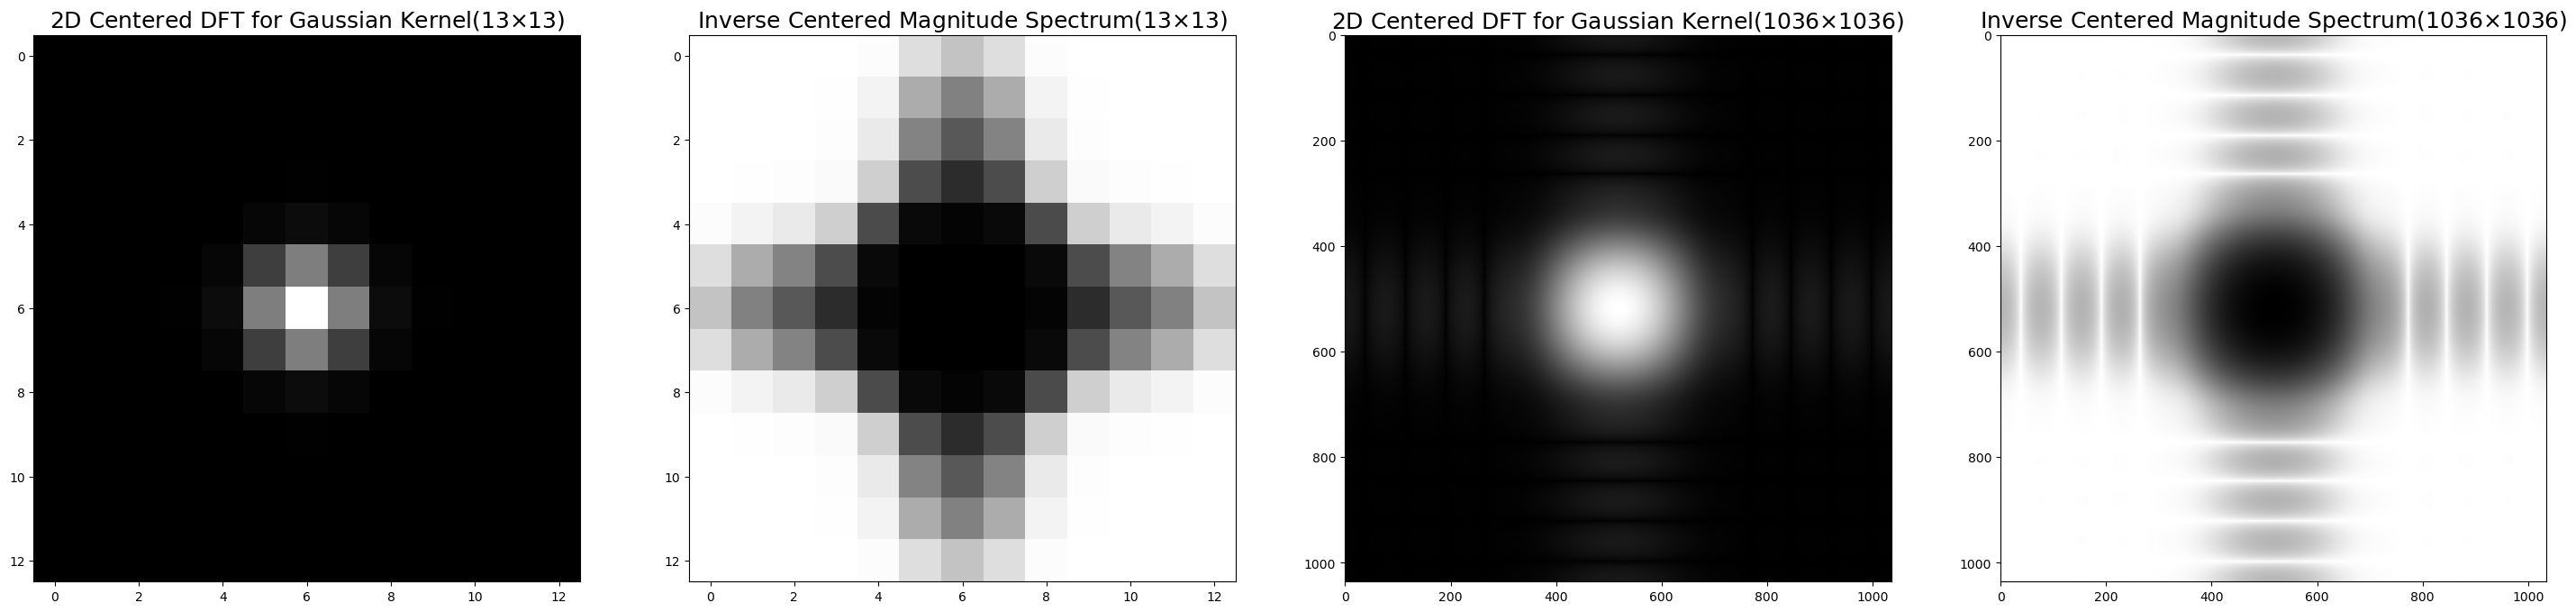
\includegraphics[scale = .18]{Output_Images/P02b.png}
        \caption{(From left) (i) Centered $13 \times 13$ kernel (ii) Centered Inverse $13 \times 13$ kernel (iii) Centered padded $1036 \times 1036$ kernel (iv) Inverse centered padded $1036 \times 1036$ kernel }
        \label{fig:2b}
        \end{figure}

        \begin{figure}[H]
        \centering
        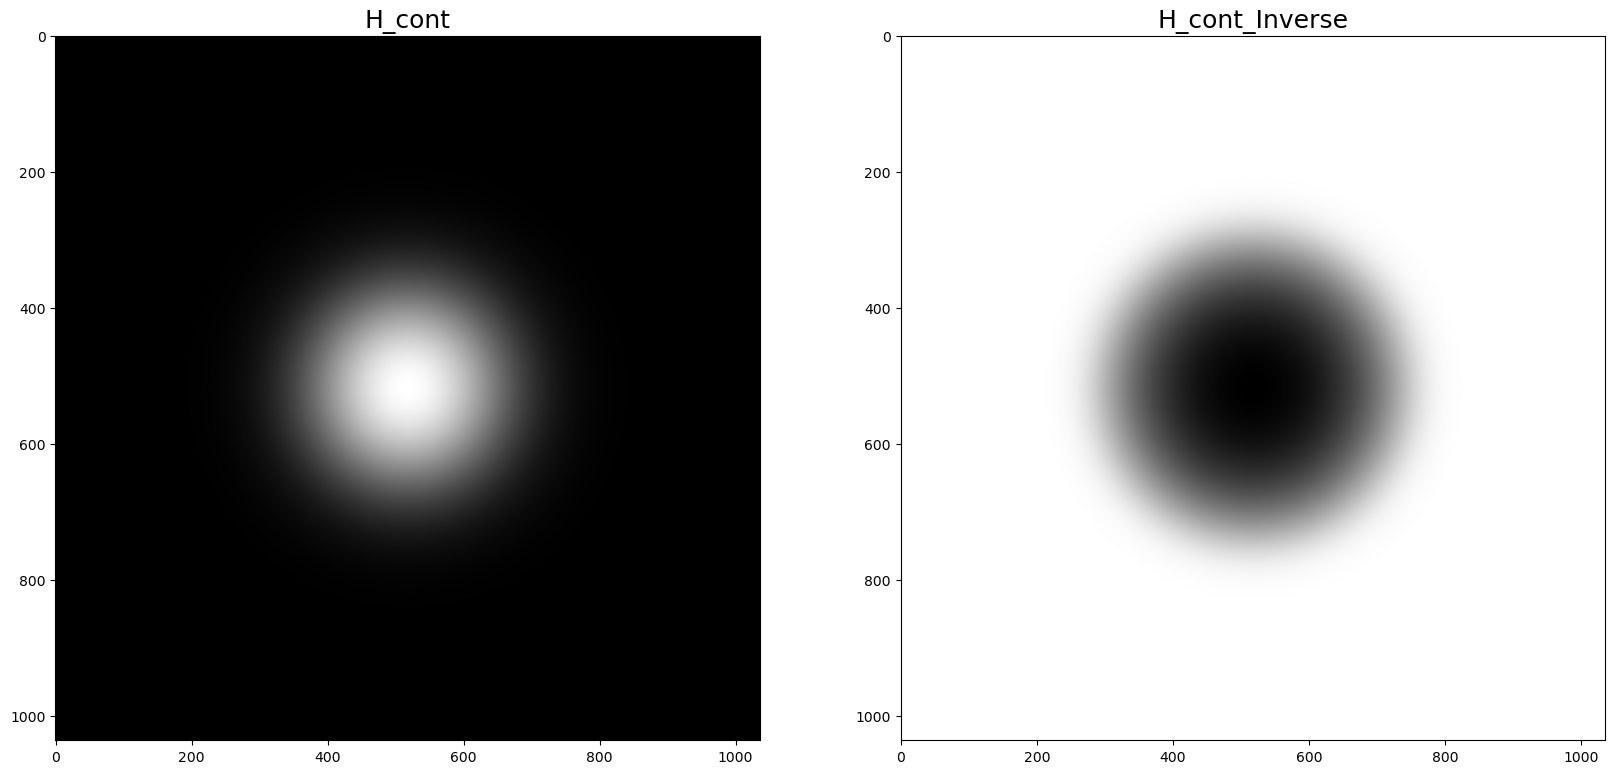
\includegraphics[scale = .18]{Output_Images/P02c.png}
        \caption{(From left) (i) Gaussian Fit (ii) Inverse Gaussian Fit}
        \label{fig:2c}
        \end{figure}
    
        \item[(d)] Finally, the restored image with both the filter is plotted in Fig.\ref{fig:2d}. The MSE of the images are as follows:
        \[        \text{MSE}_{H_{DFT}} = 0.00266, \quad
        \text{MSE}_{H_{cont}} = 0.01092\]
        The MSE of the image restored with Gaussian fit is poorer as per MSE. Also, visually there are artifacts visible in the border of the Gaussian fit images. The reason is simple that the image blurred with a filter with ripples cannot be deblurred using a smooth filter with no ripples. Evidently, there will be ripples that will come up in the final image because those are not cancelled in the frequency domain. Ripples are visible across the image when zoomed.
        \begin{figure}[H]
        \centering
        \includegraphics[scale = .18]{Output_Images/P02d.png}
        \caption{(From left) (i) Original Image; (ii) Restored Image using original inverse filter; (iii) Restored Image using Gaussian Fit filter}
        \label{fig:2d}
        \end{figure}
  \end{itemize}
\end{solution}












\end{document}